%% LyX 2.3.6 created this file.  For more info, see http://www.lyx.org/.
%% Do not edit unless you really know what you are doing.
\documentclass[english]{article}
\usepackage[T1]{fontenc}
\usepackage[latin9]{inputenc}
\usepackage{babel}
\usepackage{amssymb}
\usepackage{graphicx}
\usepackage[unicode=true]
 {hyperref}
\begin{document}
\title{ADPCM Amplification}
\maketitle

\section{Introduction}

Before being mixed to the audio left and right signals, the ADPCM
signal generated by the M5205 is biased and shrunk, re-amplified and
goes through a few low pass filters.
\begin{figure}
\caption{ADPCM Filter Circuit}

\begin{centering}
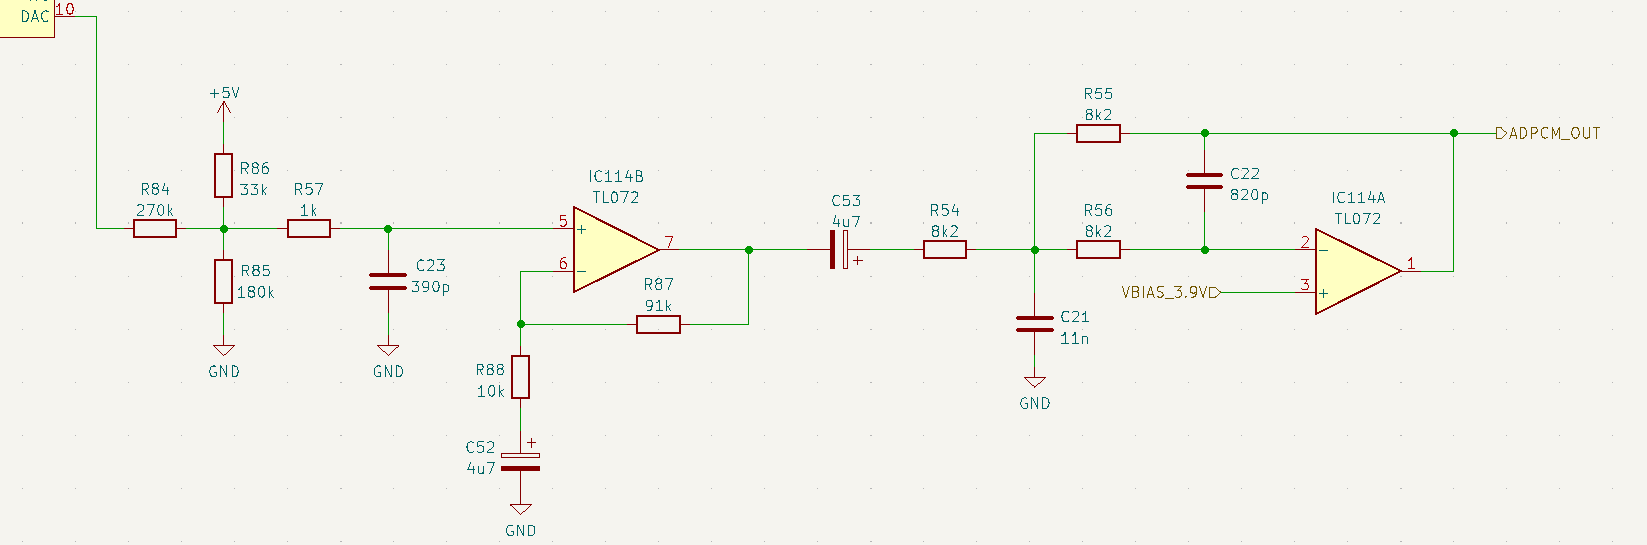
\includegraphics{adpcm}
\par\end{centering}
\end{figure}


\section{Biasing}

\begin{figure}
\caption{Biasing and Passive Low-pass Filter}

\begin{centering}
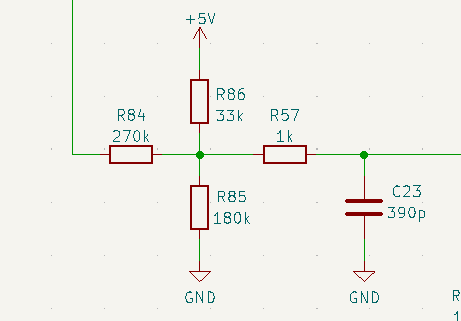
\includegraphics{biasing_passivelowpass}
\par\end{centering}
\end{figure}
The biasing is introducted by the R86 and R85 bridge divider connected
to 5V (see Figure 2). We will start with the calculation of the Thevenin
equivalent circuit at R85.

\[
V_{TH_{R85}}=\frac{V_{DAC}/R84+5V/R86+0/R85}{1/R84+1/R86+1/R85}=\frac{V_{DAC}/270k+5/33k}{1/270k+1/33k+1/180k}
\]

\[
V_{TH_{R85}}=\frac{V_{DAC}}{10.682}+3.83V
\]

\[
R_{TH_{R85}}=R84//R86//R85=\frac{1}{1/R84+1/R86+1/R85}=\frac{1}{1/270k+1/33k+1/180k}=25.277k\Omega
\]
As you can see, the DAC output is divided by 10.682 so the signal
is greatly shrunk by the biasing circuit and it is shifted up by 3.83V.

\section{Passive Low-pass filter}

Now that we have determined the Thevenin equivalent, we can calculate
the low pass filter including R57 and C23.

\[
V_{C23}=\frac{Z_{C23}}{R_{TH_{R85}}+R57+Z_{C23}}\times V_{TH_{R85}}=\frac{1/jC23\omega}{R_{TH_{R85}}+R57+1/jC23\omega}\times V_{TH_{R85}}
\]

\[
V_{C23}=\frac{1}{1+j\left(R_{TH_{R85}}+R57\right)C23\omega}\times V_{TH_{R85}}
\]
\linebreak{}
At DC level, when $j\omega=0$, C23 acts an open circuit and therefore
$V_{TH_{R85}}$ is applied directly to V+. $V_{TH_{R85}}$ will include
3.83V and DC bias added in software to VDAC which is typically 2.5V.
Since VDAC is divided by 10.682, a 2.5V DC offset will give 0.234V.
$V_{TH_{R85}}=3.83+0.234\thickapprox4V$\linebreak{}
\linebreak{}
Let's now work out the cut-off frequency of the low-pass filter.

\[
\omega_{C}=\frac{1}{(R_{TH_{R85}}+R57)C23}\rightarrow f_{C}=\frac{1}{2\pi(R_{TH_{R85}}+R57)C23}=\frac{1}{2\pi\times(25.277k+1k)\times390\times10^{-12}}=15538Hz
\]
\linebreak{}
First order filter with -3dB attenuation at $f_{c}=15538Hz$ and -20dB
per decade.

\section{IC114B - Positive Gain Amplifier}

\begin{figure}
\begin{centering}
\caption{Positive Gain Amplifier}
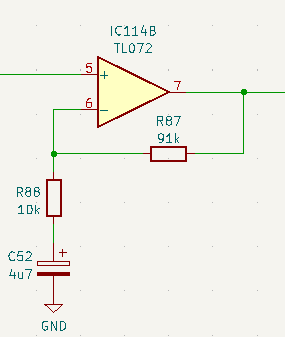
\includegraphics{positivegain_opamp}
\par\end{centering}
\end{figure}
IC114B has a negative feedback and the input voltage is connected
to the positive input. Therefore it is configured as an amplifier
with a positive gain. C52 is a fairly large capacitor connected to
ground which ensure gain is only applied at AC level where the opamp
becomes a simple follower at DC level. In other words, the ADPCM signal
is amplified and bias voltage is preserved.\linebreak{}
\linebreak{}
At DC level, when $j\omega=0$, C52 is seen as an open circuit therefore:
\[
V_{IC114B+}=V_{R85}=V_{IC114B-}=V_{IC114BOUT}=4V
\]
AC level, IC114B acts as positive gain amplifer.

\[
V_{IC114B-}=\frac{R88+1/jC52\omega}{R88+1/jC52\omega+R87}\times V_{IC114BOUT}
\]
\linebreak{}
When $j\omega\rightarrow\infty$, capacitors be come short circuits
and we can determine the gain for high frequencies.

\[
V_{IC114B-}=\frac{R88}{R88+R87}\times V_{IC114BOUT}=V_{IC114B+}=V_{R85AC}
\]

\[
Gain=\frac{V_{IC114BOUT}}{V_{R85AC}}=\frac{R88+R87}{R88}=\frac{10k+91k}{10k}=10.1
\]

\[
\frac{V_{IC114BOUT}}{V_{R85AC}}=\frac{R88+1/jC52\omega+R87}{R88+1/jC52\omega}=\frac{1+j(R87+R88)\times C52\omega}{1+jR88C52\omega}
\]
\linebreak{}
To determine the cut frequency of the high-pass filter we know that
gain must be 3dB away from the final final. i.e. $10.1/\sqrt{2}=7.142$

\[
\left|\frac{V_{IC114BOUT}}{V_{R85AC}}\right|=\frac{\left|1+j(R87+R88)\times C52\omega\right|}{\left|1+jR88C52\omega\right|}=\frac{\left|1+j0.4747\omega\right|}{\left|1+j0.047\omega\right|}=\frac{\sqrt{1+0.4747^{2}\omega^{2}}}{\sqrt{1+0.047^{2}\omega^{2}}}
\]

\[
\frac{1+0.4747^{2}\omega_{C}^{2}}{1+0.047^{2}\omega_{C}^{2}}=7.142^{2}=51
\]
\[
1+0.4747^{2}\omega_{C}^{2}=51\times\left(1+0.047^{2}\omega_{C}^{2}\right)
\]

\[
0.4747^{2}\omega_{C}^{2}-51\times0.047^{2}\omega_{C}^{2}=51-1
\]

\[
\omega_{C}^{2}\left(0.4747^{2}-51\times0.047^{2}\right)=50
\]

\[
\omega_{C}=\sqrt{\frac{50}{\left(0.4747^{2}-51\times0.047^{2}\right)}}=21.065
\]
\linebreak{}
It is now possible to work out the cut frequency of the high-pass
filter. 
\[
f_{C}=\frac{\omega_{C}}{2\pi}=\frac{21.065}{2\times3.14}=3.354Hz
\]


\section{IC114A - Multi-Feedback Amplifier}

\begin{figure}

\caption{Multi-Feeback Amplifier}

\begin{centering}
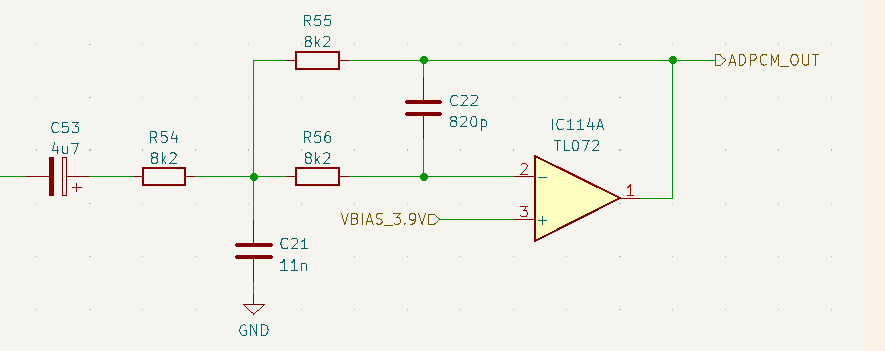
\includegraphics{mfb_opamp}
\par\end{centering}
\end{figure}
This opamp is configured as an MFB (multi-feedback) filter which is
a second order low-pass filter but also no gain at DC. For the calculations,
C53 is removed but its purpose is to remove any DC offset before it
is fed to the opamp.\linebreak{}
\linebreak{}
When $j\omega=0$, C53, C21 and C22 act as open circuits. Therefore:

\[
V_{IC114A-}=V_{ADPCMOUT}=V_{IC114B+}=V_{BIAS}=3.90V
\]
When $j\omega\rightarrow\infty$, C22 is a short circuit turning IC114A
into a follower but at this stage C21 is shorting the input signal
to ground so there will be no high-frequency output signal.\linebreak{}
\linebreak{}
To find the transfer function of this opamp circuit, we will break
in down in 2 stages: calculation of voltage at C21 and then calculation
of voltage at IC114A-. To simplify calulations, VBIAS biased will
be switched off to make $V_{IC114A-}=V_{IC114A+}=0V$. With this simplification,
the connection R56 and C22 will be tied to GND. \linebreak{}
\linebreak{}
\[
V_{C21}=\frac{\frac{V_{IC114BOUT}}{R54}+\frac{V_{ADPCMOUT}}{R55}}{\frac{1}{R54}+\frac{1}{R55}+\frac{1}{R56}+jC21\omega}
\]

\[
V_{IC114A-1}=\frac{\frac{V_{ADPCMOUT}}{1/jC22\omega}+\frac{V_{C21}}{R56}}{jC22\omega+\frac{1}{R56}}=0
\]

\[
V_{C21}=-jR56C22\omega\times V_{ADPCMOUT}
\]

\[
\frac{\frac{V_{IC114BOUT}}{R54}+\frac{V_{ADPCMOUT}}{R55}}{\frac{1}{R54}+\frac{1}{R55}+\frac{1}{R56}+jC21\omega}=-jR56C22\omega\times V_{ADPCMOUT}
\]

\[
\frac{V_{IC114BOUT}}{R54}+\frac{V_{ADPCMOUT}}{R55}=-jR56C22\omega\times V_{ADPCMOUT}\times\left(\frac{1}{R54}+\frac{1}{R55}+\frac{1}{R56}+jC21\omega\right)
\]

\[
V_{ADPCMOUT}\times\left(\frac{1}{R55}+jR56C22\omega\times\left(\frac{1}{R54}+\frac{1}{R55}+\frac{1}{R56}+jC21\omega\right)\right)=-\frac{V_{IC114BOUT}}{R54}
\]

\[
\frac{V_{ADPCMOUT}}{V_{IC114BOUT}}=-\frac{1}{R54}\times\frac{1}{\frac{1}{R55}+jR56C22\omega\times\left(\frac{1}{R54}+\frac{1}{R55}+\frac{1}{R56}+jC21\omega\right)}
\]

\[
\frac{V_{ADPCMOUT}}{V_{IC114BOUT}}=-\frac{1}{R54R56}\times\frac{1}{\frac{1}{R55R56}+jC22\omega\times\frac{R55R56+R54R56+R54R55}{R54R55R56}-C21C22\omega^{2}}
\]

\[
\frac{V_{ADPCMOUT}}{V_{IC114BOUT}}=-\frac{1}{R54R56C21C22}\times\frac{1}{\frac{1}{R55R56C21C22}+j\frac{R55R56+R54R56+R54R55}{R54R55R56C21}\omega-\omega^{2}}
\]
\linebreak{}
Since R54=R55=R56, we will replace them with R instead to simplify
the equation:

\[
\frac{V_{ADPCMOUT}}{V_{IC114BOUT}}=-\frac{1}{R^{2}C21C22}\times\frac{1}{\frac{1}{R^{2}C21C22}+j\frac{R^{2}+R^{2}+R^{2}}{R^{3}C21}\omega-\omega^{2}}=-\frac{1}{R^{2}C21C22}\times\frac{1}{\frac{1}{R^{2}C21C22}+j\frac{3}{RC21}\omega-\omega^{2}}
\]

\[
H\left(j\omega\right)=-\frac{1}{1+j3RC22\omega-R^{2}C21C22\omega^{2}}
\]
\linebreak{}
Now that we have the transfer function, we can see that when $j\omega=0$,
the DC gain is 1. \linebreak{}
\linebreak{}
\[
\omega_{C}=\frac{1}{\sqrt{R^{2}C21C22}};\omega_{C}=2\pi f_{C};f_{C}=\frac{1}{2\times\pi\times\sqrt{8.2k\times8.2k\times11\times10^{-9}\times390\times10^{-12}}}=6463Hz
\]
\linebreak{}
The cut-off freuqency is 6463Hz and -40dB percade will be applied
by the filter. The next stage is the Quality factor calculation but
I can't remember how to do that. To get the value, I typed the component
values in \href{http://sim.okawa-denshi.jp/en/OPttool.php}{this link}
and it gave me Q=1.2209.
\end{document}
